
\chapter{{Direct Attack on MQ using CDCL SAT solvers}}
\label{chap:MPQC}
%\section{Secure Parameters against HybridF5 attack}
In this chapter, we are going to review the best known structural attacks  against the ABC, UOV and Rainbow multivariate schemes. These known best structural attacks to each specific scheme together the HybridF5 attack given secure parameters which we are going to use to construct several instances of these schemes and attack them using CDCL SAT solvers. 

Specifically, we used a massively parallel portfolio SAT solver called HordeSAT which used MPI. As we said, the SAT solvers in the portfolio can be instances of a single solver with different configuration settings. Additionally the solvers can exchange information usually in the form of clauses.
\section{UOV}
Taking into account the attack of \cite{Thomae2012} and using the equations \eqref{eq:complexdetermined_gf16},\eqref{eq:complexdetermined_gf31} and \eqref{eq:complexdetermined_gf256} \cite{AlbrechtPetzoldt2013} has calculated the secure parameters for the Rainbow and UOV schemes. Because of the attack of \cite{Thomae2012} reduce the number of equations in the public systems by 2 before applying an algorithm like HybridF5, \cite{AlbrechtPetzoldt2013} increased the number of equations by 2. Besides, to defend the scheme against the
UOV attack of \cite{Kipnis1999}, they recommend choose $v=2\cdot o$. Thus, in the Table \ref{table:security_level_uov} are shown the proposed parameter sets for the UOV scheme for different levels of security and different underlying fields.

\begin{table}
\centering
\caption{UOV parameters and security level for $\mathbb{F}_{16}$, $\mathbb{F}_{31}$ and $\mathbb{F}_{256}$}
\label{table:security_level_uov}
\begin{tabular}{|c|c|c|c|c|c|c|}
\hline
\multicolumn{1}{|c|}{}                     & \multicolumn{2}{c|}{$\mathbb{F}_{16}$}            & \multicolumn{2}{c|}{$\mathbb{F}_{31}$}            & \multicolumn{2}{c|}{$\mathbb{F}_{256}$}           \\ \hline
\multicolumn{1}{|c|}{security level (bit)} & \multicolumn{1}{c|}{$o$} & \multicolumn{1}{c|}{$v$} & \multicolumn{1}{c|}{$o$} & \multicolumn{1}{c|}{$v$} & \multicolumn{1}{c|}{$o$} & \multicolumn{1}{c|}{$v$} \\ \hline
16 & 3 & 6 & 3 & 6 & 3 & 6 \\ \hline
17 & 3 & 6 & 4 & 8 & 4 & 8 \\ \hline
18 & 4 & 8 & 4 & 8 & 4 & 8 \\ \hline
19 & 4 & 8 & 4 & 8 & 5 & 10 \\ \hline
20 & 4 & 8 & 5 & 10 & 5 & 10 \\ \hline
21 & 5 & 10 & 5 & 10 & 5 & 10 \\ \hline
22 & 5 & 10 & 6 & 12 & 6 & 12 \\ \hline
23 & 6 & 12 & 6 & 12 & 6 & 12 \\ \hline
24 & 6 & 12 & 6 & 12 & 6 & 12 \\ \hline
25 & 7 & 14 & 7 & 14 & 7 & 14 \\ \hline
26 & 7 & 14 & 7 & 14 & 7 & 14 \\ \hline
27 & 7 & 14 & 8 & 16 & 8 & 16 \\ \hline
28 & 8 & 16 & 8 & 16 & 8 & 16 \\ \hline
29 & 8 & 16 & 8 & 16 & 8 & 16 \\ \hline
30 & 9 & 18 & 9 & 18 & 9 & 18 \\ \hline
31 & 9 & 18 & 9 & 18 & 9 & 18 \\ \hline
32 & 10 & 20 & 10 & 20 & 10 & 20 \\ \hline
33 & 10 & 20 & 10 & 20 & 10 & 20 \\ \hline
34 & 11 & 22 & 10 & 20 & 10 & 20 \\ \hline
35 & 11 & 22 & 11 & 22 & 11 & 22 \\ \hline
36 & 11 & 22 & 11 & 22 & 11 & 22 \\ \hline
37 & 12 & 24 & 12 & 24 & 11 & 22 \\ \hline
38 & 12 & 24 & 12 & 24 & 12 & 24 \\ \hline
39 & 13 & 26 & 12 & 24 & 12 & 24 \\ \hline
40 & 13 & 26 & 13 & 26 & 13 & 26 \\ \hline
41 & 14 & 28 & 13 & 26 & 13 & 26 \\ \hline
42 & 14 & 28 & 14 & 28 & 13 & 26 \\ \hline
43 & 14 & 28 & 14 & 28 & 14 & 28 \\ \hline
44 & 15 & 30 & 14 & 28 & 14 & 28 \\ \hline
\end{tabular}
\end{table}

\noindent
\textbf{Solving UOV intances over $\mathbb{F}_{16}$ using CDCL SAT solvers}
\begin{table}[]
\centering
\caption{HordeSAT configurations}
\label{my-label}
\begin{tabular}{lccccc}
\hline
\multicolumn{1}{l|}{Core Solvers} & \multicolumn{1}{c|}{Parallel Solved} & \multicolumn{1}{c|}{Avg.} & \multicolumn{1}{c|}{Tot.} & \multicolumn{1}{c}{Med} \\ \hline
solved-lingeling\_uov\_1x6x4 & 150 & 1 & 1.00 & 1.00 \\\hline
solved-lingeling\_uov\_2x6x4 & 150 & 3 & 1.68 & 1.12  \\\hline
solved-lingeling\_uov\_4x6x4 & 150 & 4 & 2.15 & 1.49 \\\hline
solved-lingeling\_uov\_8x6x4 & 150  & 14 & 6.39 & 2.83 \\\hline
solved-lingeling\_uov\_16x6x4 & 150  & 13 & 11.70 & 2.45  \\\hline
solved-lingeling\_uov\_32x6x4 & 150 & 12 & 17.46 & 2.86 \\\hline
solved-lingeling\_uov\_64x6x4 & 150 & 15 & 20.64 & 2.36 \\\hline
solved-lingeling\_uov\_128x6x4 & 150 & 19 & 25.22 & 2.10 \\\hline
solved-lingeling\_uov\_256x6x4 & 150  & 10 & 14.41 & 1.33  \\\hline
solved-lingeling\_uov\_512x6x4 & 150  & 18 & 21.37 & 1.36  \\\hline
\end{tabular}
\end{table}



\section{ABC}
Following the model showed in \cite{AlbrechtPetzoldt2013} we have calculated the secure parameters for the ABC scheme proposed by \cite{Tao2015}. Taking into account that the attack of \cite{Thomae2012}  reduce the number of equations in the public systems by 2 before applying an algorithm like HybridF5, we increased the number of equations by 2. Also, the known best structural attack against this scheme was proposed by \cite{Moody2014} and its complexity is 
\begin{equation}
s^6\cdot q^{s+4}
\label{eq:structural}
\end{equation}
for even characteristic and 
\begin{equation}
s^6\cdot q^{s+2}
\end{equation} for odd characteristic. 
%In this thesis, we have to study secure parameters of the ABC scheme constructed over finite fields with even characteristic.
Hereafter, we are going to name StructuralABC the attack proposed by \cite{Moody2014}. 

We use the equations \eqref{eq:complexityHF5w} and \eqref{eq:structural} to make a comparison between the complexity of the HybridF5 and StructuralABC attacks against instances of the ABC cryptosystem over $\mathbb{F}_2$, $\mathbb{F}_4$, $\mathbb{F}_{16}$ and $\mathbb{F}_{256}$. Figures \ref{fig:hybridF5_structural_gf2}, \ref{fig:hybridF5_structural_gf4}, \ref{fig:hybridF5_structural_gf16} and \ref{fig:hybridF5_structural_gf256} show the results when the equations \eqref{eq:complexityHF5w} and \eqref{eq:structural} are evaluated for $m \in \{8,\cdots,108\}$.\footnote{for the case of the HybridF5 was chose the minimum k - note by Juan}.

Clearly figure \ref{fig:hybridF5_structural_gf256} shows that the best attack is the HybridF5 for those values of $m$. However, in figures \ref{fig:hybridF5_structural_gf2}, \ref{fig:hybridF5_structural_gf4} and \ref{fig:hybridF5_structural_gf16} are showed that there is not a absolute best attack for those chosen values of $m$. Thus, to be more precise and determine which is the intersection point that define at which interval the best attack is HybridF5 or StructuralABC, we have to re-write the equations \eqref{eq:HF5_gf2_4}, \eqref{eq:HF5_gf16} and  \eqref{eq:HF5_gf256} for the critic intervals. Evaluating the equation \eqref{eq:complexityHF5w} for the critic values, we find that the bit complexity of the HybridF5 attack against instances of the ABC scheme with $m$ multivariate quadratic equations and $n$ variables is roughly
%GF2,GF4:m=1...7;GF16:m=18...24
\begin{equation}
0.72\cdot m+ 3.45
\end{equation}
for system over $\mathbb{F}_2$,
\begin{equation}
1.28\cdot m + 2.45
\end{equation}
for system over $\mathbb{F}_4$,
\begin{equation}
0.77\cdot m + 11.62
\end{equation}
for system over $\mathbb{F}_{16}$,

On other hand, evaluating \eqref{eq:structural} for $m\in \{8,\cdots,108\}$, we find that the bit complexity of the StructuralABC attack against instances of the ABC scheme with $m$ multivariate quadratic equations and $n$ variables is roughly
\begin{equation}0.15\cdot m + 14.56\label{eq:structuralgf2}\end{equation}
for system over $\mathbb{F}_2$,
\begin{equation}0.19\cdot m + 20.9\label{eq:structuralgf4}\end{equation}
for system over $\mathbb{F}_4$,
\begin{equation}0.29\cdot m + 33.42\label{eq:structuralgf16}\end{equation}
for system over $\mathbb{F}_{16}$,
\begin{equation}0.5\cdot m + 58.47\label{eq:structuralgf256}\end{equation}
for system over $\mathbb{F}_{256}$.

Thus, according this comparison, we find 
\begin{itemize}
\item for instances of the ABC scheme over $\mathbb{F}_2$ the known best attack is the HybridF5 attack, if  $m\leq 19$ and the StructuralABC if $m\geq 20$,
\item for instances of the ABC scheme over $\mathbb{F}_4$ the known best attack is the HybridF5 attack, if  $m\leq 17$ and the StructuralABC if $m\geq 18$,
\item for instances of the ABC scheme over $\mathbb{F}_16$ the known best attack is the HybridF5 attack, if  $m\leq 45$ and the StructuralABC if $m\geq 46$,
\item for instances of the ABC scheme over $\mathbb{F}_{256}$ the known best attack is the HybridF5 attack for all considered cases of $m$.
\end{itemize}

\begin{figure}
\centering
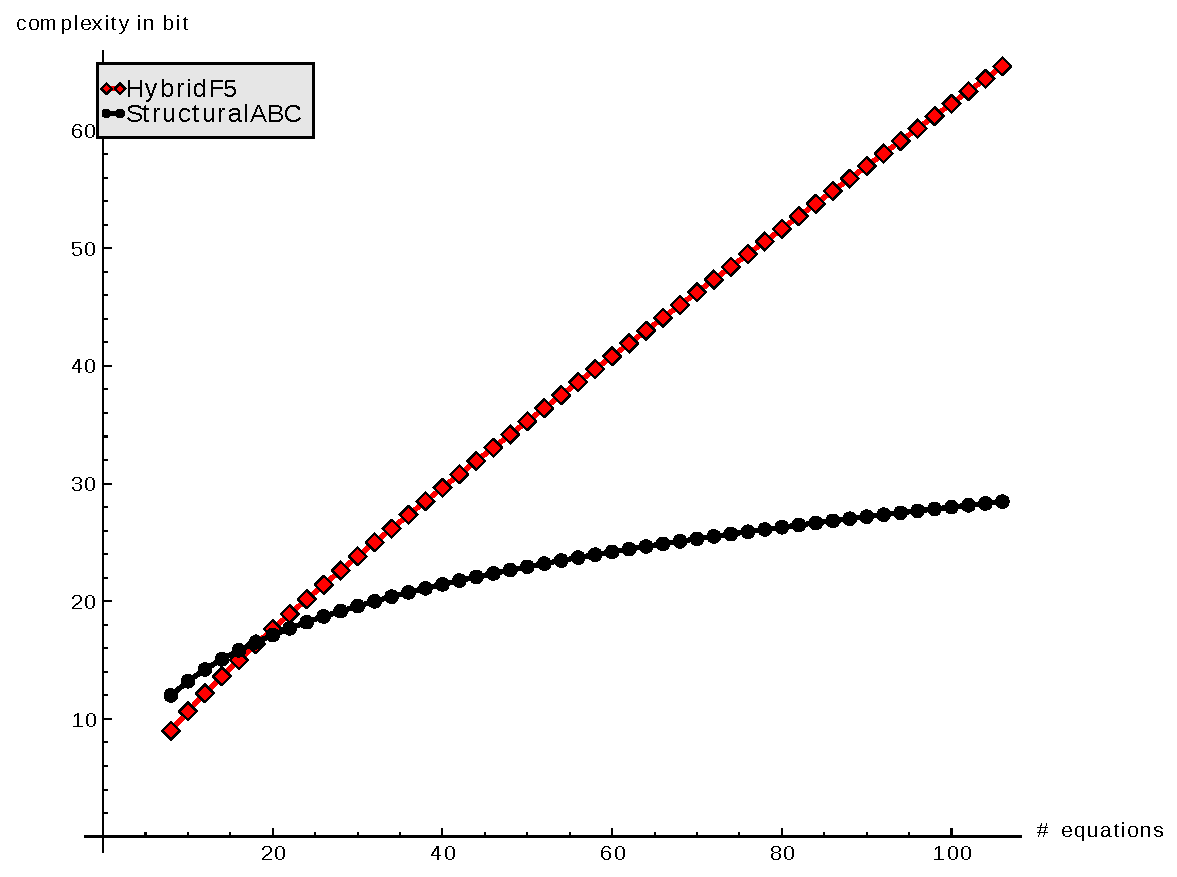
\includegraphics[width=10cm]{figures/hybridF5_structural_vs_m_gf2.pdf}
\caption{Complexity of the HybridF5 and StructuralABC attacks against instances of the ABC cryptosystem over $\mathbb{F}_2$.}
\label{fig:hybridF5_structural_gf2}
\end{figure}

\begin{figure}
\centering
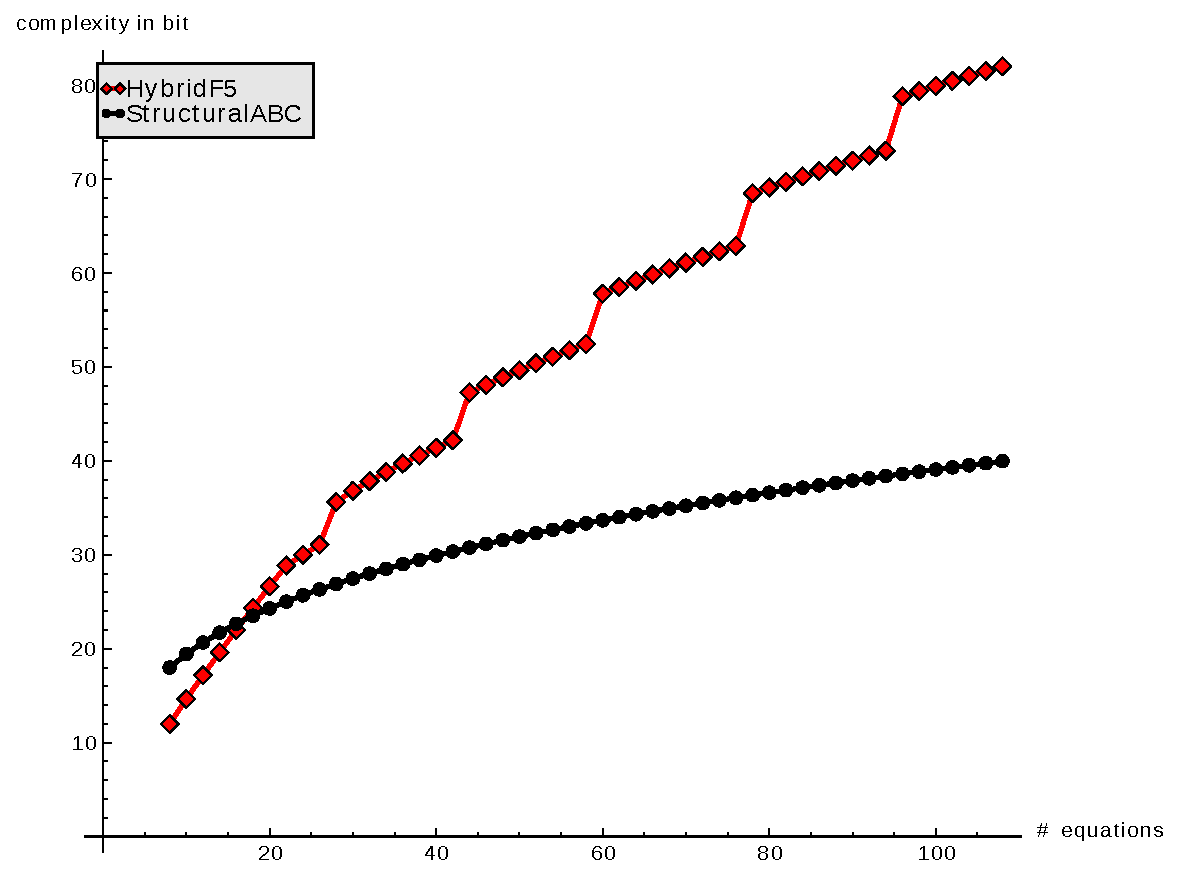
\includegraphics[width=10cm]{figures/hybridF5_structural_vs_m_gf4.pdf}
\caption{Complexity of the HybridF5 and StructuralABC attacks against instances of the ABC cryptosystem over $\mathbb{F}_4$.}
\label{fig:hybridF5_structural_gf4}
\end{figure}

\begin{figure}
\centering
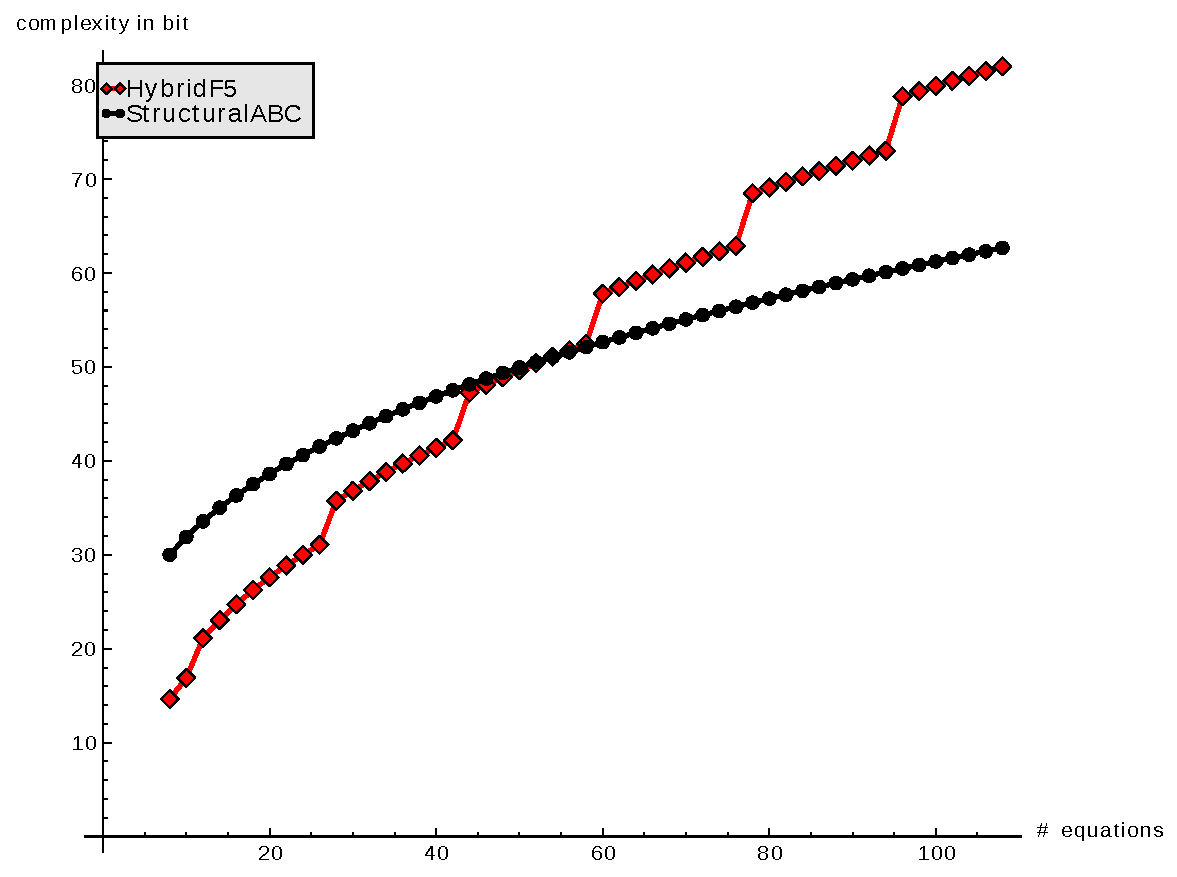
\includegraphics[width=10cm]{figures/hybridF5_structural_vs_m_gf16.pdf}
\caption{Complexity of the HybridF5 and StructuralABC attacks against instances of the ABC cryptosystem over $\mathbb{F}_{16}$.}
\label{fig:hybridF5_structural_gf16}
\end{figure}


\begin{figure}
\centering
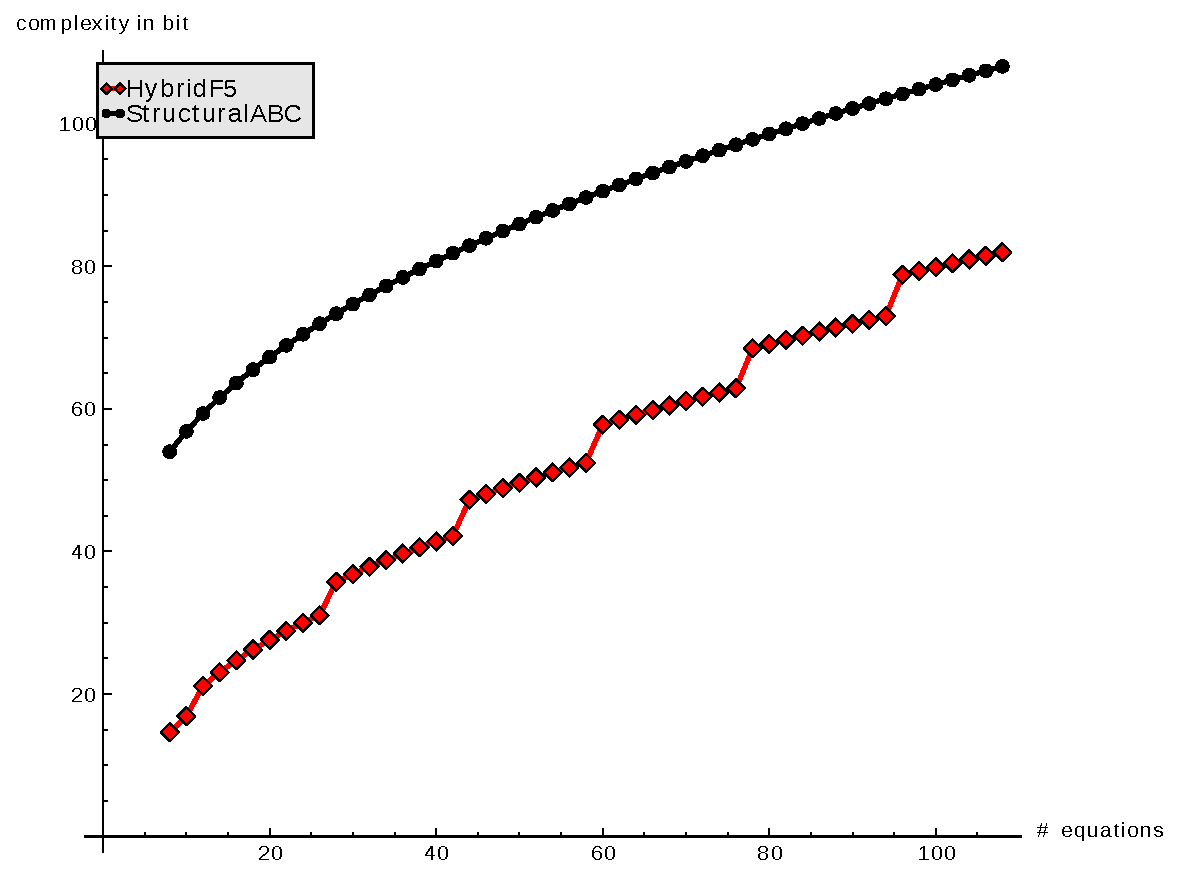
\includegraphics[width=10cm]{figures/hybridF5_structural_vs_m_gf256.pdf}
\caption{Complexity of the HybridF5 and StructuralABC attacks against instances of the ABC cryptosystem over $\mathbb{F}_{256}$.}
\label{fig:hybridF5_structural_gf256}
\end{figure}
In the Table \ref{table:security_level_abc} are shown the proposed parameter sets for the ABC scheme for different levels of security and different underlying fields.

\begin{table}[]
\centering
\caption{My caption}
\label{my-label}
\begin{tabular}{|c|c|c|c|c|}
\hline
                    & $\mathbb{F}_2$           & $\mathbb{F}_4$           & $\mathbb{F}_{16}$          & $\mathbb{F}_{256}$         \\ \hline
security level(bit) & \multicolumn{1}{c|}{$s$} & \multicolumn{1}{c|}{$s$} & \multicolumn{1}{c|}{$s$} & \multicolumn{1}{c|}{$s$} \\ \hline
16 &$\sqrt{ 10 }$&$\sqrt{ 7 }$&$\sqrt{ 4 }$&$\sqrt{ 3/2 }$\\ \hline
17 &$\sqrt{ 11 }$&$\sqrt{ 7 }$&$\sqrt{ 9/2 }$&$\sqrt{ 5/2 }$\\ \hline
18 &$\sqrt{ 13 }$&$\sqrt{ 7 }$&$\sqrt{ 5 }$&$\sqrt{ 3 }$\\ \hline
19 &$\sqrt{ 16 }$&$\sqrt{ 8 }$&$\sqrt{ 6 }$&$\sqrt{ 4 }$\\ \hline
20 &$\sqrt{ 19 }$&$\sqrt{ 8 }$&$\sqrt{ 13/2 }$&$\sqrt{ 9/2 }$\\ \hline
21 &$\sqrt{ 23 }$&$\sqrt{ 8 }$&$\sqrt{ 7 }$&$\sqrt{ 11/2 }$\\ \hline
22 &$\sqrt{ 26 }$&$\sqrt{ 9 }$&$\sqrt{ 15/2 }$&$\sqrt{ 6 }$\\ \hline
23 &$\sqrt{ 29 }$&$\sqrt{ 9 }$&$\sqrt{ 17/2 }$&$\sqrt{ 7 }$\\ \hline
24 &$\sqrt{ 33 }$&$\sqrt{ 10 }$&$\sqrt{ 9 }$&$\sqrt{ 15/2 }$\\ \hline
25 &$\sqrt{ 36 }$&$\sqrt{ 12 }$&$\sqrt{ 19/2 }$&$\sqrt{ 17/2 }$\\ \hline
26 &$\sqrt{ 39 }$&$\sqrt{ 15 }$&$\sqrt{ 21/2 }$&$\sqrt{ 9 }$\\ \hline
27 &$\sqrt{ 43 }$&$\sqrt{ 17 }$&$\sqrt{ 11 }$&$\sqrt{ 10 }$\\ \hline
28 &$\sqrt{ 46 }$&$\sqrt{ 20 }$&$\sqrt{ 23/2 }$&$\sqrt{ 21/2 }$\\ \hline
29 &$\sqrt{ 49 }$&$\sqrt{ 23 }$&$\sqrt{ 25/2 }$&$\sqrt{ 23/2 }$\\ \hline
30 &$\sqrt{ 53 }$&$\sqrt{ 25 }$&$\sqrt{ 13 }$&$\sqrt{ 25/2 }$\\ \hline
31 &$\sqrt{ 56 }$&$\sqrt{ 28 }$&$\sqrt{ 27/2 }$&$\sqrt{ 13 }$\\ \hline
32 &$\sqrt{ 59 }$&$\sqrt{ 30 }$&$\sqrt{ 14 }$&$\sqrt{ 14 }$\\ \hline
33 &$\sqrt{ 63 }$&$\sqrt{ 33 }$&$\sqrt{ 15 }$&$\sqrt{ 29/2 }$\\ \hline
34 &$\sqrt{ 66 }$&$\sqrt{ 36 }$&$\sqrt{ 31/2 }$&$\sqrt{ 31/2 }$\\ \hline
35 &$\sqrt{ 69 }$&$\sqrt{ 38 }$&$\sqrt{ 16 }$&$\sqrt{ 16 }$\\ \hline
36 &$\sqrt{ 73 }$&$\sqrt{ 41 }$&$\sqrt{ 17 }$&$\sqrt{ 17 }$\\ \hline
37 &$\sqrt{ 76 }$&$\sqrt{ 44 }$&$\sqrt{ 35/2 }$&$\sqrt{ 35/2 }$\\ \hline
38 &$\sqrt{ 79 }$&$\sqrt{ 46 }$&$\sqrt{ 18 }$&$\sqrt{ 37/2 }$\\ \hline
39 &$\sqrt{ 83 }$&$\sqrt{ 49 }$&$\sqrt{ 19 }$&$\sqrt{ 19 }$\\ \hline
40 &$\sqrt{ 86 }$&$\sqrt{ 52 }$&$\sqrt{ 39/2 }$&$\sqrt{ 20 }$\\ \hline
41 &$\sqrt{ 89 }$&$\sqrt{ 54 }$&$\sqrt{ 20 }$&$\sqrt{ 41/2 }$\\ \hline
42 &$\sqrt{ 93 }$&$\sqrt{ 57 }$&$\sqrt{ 41/2 }$&$\sqrt{ 43/2 }$\\ \hline
43 &$\sqrt{ 96 }$&$\sqrt{ 59 }$&$\sqrt{ 43/2 }$&$\sqrt{ 45/2 }$\\ \hline
44 &$\sqrt{ 99 }$&$\sqrt{ 62 }$&$\sqrt{ 22 }$&$\sqrt{ 23 }$\\ \hline
\end{tabular}
\end{table}

\begin{table}[]
\centering
\caption{$\mathbb{F}_{16}$ }
\label{my-label}
\begin{tabular}{|c|c|c|c|c|}
\hline
                    & $\mathbb{F}_2$           & $\mathbb{F}_4$           & $\mathbb{F}_{16}$          & $\mathbb{F}_{256}$         \\ \hline
security level(bit) & \multicolumn{1}{c|}{$s$} & \multicolumn{1}{c|}{$s$} & \multicolumn{1}{c|}{$s$} & \multicolumn{1}{c|}{$s$} \\  \hline
18 &$\sqrt{ 25/2 }$&$\sqrt{ -13/2 }$&$\sqrt{ 3 }$&$\sqrt{ 3 }$\\ \hline
19 &$\sqrt{ 16 }$&$\sqrt{ -4 }$&$\sqrt{ 4 }$&$\sqrt{ 4 }$\\ \hline
22 &$\sqrt{ 26 }$&$\sqrt{ 4 }$&$\sqrt{ 6 }$&$\sqrt{ 6 }$\\ \hline
23 &$\sqrt{ 29 }$&$\sqrt{ 13/2 }$&$\sqrt{ 7 }$&$\sqrt{ 7 }$\\ \hline
26 &$\sqrt{ 39 }$&$\sqrt{ 29/2 }$&$\sqrt{ 9 }$&$\sqrt{ 9 }$\\ \hline
27 &$\sqrt{ 85/2 }$&$\sqrt{ 17 }$&$\sqrt{ 10 }$&$\sqrt{ 10 }$\\ \hline
31 &$\sqrt{ 56 }$&$\sqrt{ 55/2 }$&$\sqrt{ 13 }$&$\sqrt{ 13 }$\\ \hline
32 &$\sqrt{ 59 }$&$\sqrt{ 30 }$&$\sqrt{ 14 }$&$\sqrt{ 14 }$\\ \hline
35 &$\sqrt{ 69 }$&$\sqrt{ 38 }$&$\sqrt{ 16 }$&$\sqrt{ 16 }$\\ \hline
36 &$\sqrt{ 145/2 }$&$\sqrt{ 81/2 }$&$\sqrt{ 17 }$&$\sqrt{ 17 }$\\ \hline
39 &$\sqrt{ 165/2 }$&$\sqrt{ 97/2 }$&$\sqrt{ 19 }$&$\sqrt{ 19 }$\\ \hline
40 &$\sqrt{ 86 }$&$\sqrt{ 103/2 }$&$\sqrt{ 20 }$&$\sqrt{ 20 }$\\ \hline
44 &$\sqrt{ 99 }$&$\sqrt{ 62 }$&$\sqrt{ 23 }$&$\sqrt{ 23 }$\\ \hline
\end{tabular}
\end{table}
\section{Secure Parameters against SAT solving attack}


\begin{table}[]
\centering
\caption{Running Times vs Security Levels for UOV over $\mathbb{F}_{16}$ }
\scriptsize
\label{my-label}
\begin{tabular}{|c|c|c|c|c|c|c|c|c|c|c|}
\hline
security level & 1x6x4 & 2x6x4 & 4x6x4 & 8x6x4 & 16x6x4 & 32x6x4 & 64x6x4 & 128x6x4 & 256x6x4 & 512x6x4 \\ \hline

22 & 1.9492 & 1.669 & 1.2832 & 1.1602 & 1.2624 & 1.4404 & 1.761 & 2.1884 & 3.108 & 16.3644 \\ \hline
23 & 34.1918 & 18.7232 & 10.0598 & 8.357 & 6.2682 & 5.1414 & 5.5122 & 5.3082 & 12.913 & 7.5914\\ \hline
24 & 1250.32 & 741.795 & 584.909 & 191.694 & 102.364 & 67.0636 & 55.034 & 43.4934 & 73.2016 & 36.2316 \\ \hline
\end{tabular}
\end{table}


